% Länge 1:
% Länge 2:
% normale Schwingung:
% Exp L1:   T_linkes_L1: 1.237+/-0.005 in s       T_rechtes_L1: 1.238+/-0.004in s
% Exp L1 :  T_linkes_L2: 1.602+/-0.006 in s       T_rechtes_L2: 1.608+/-0.006in s
% gleichsinnige Schwingung:
% Exp L1:   T_gleich_L1: 1.194+/-0.004 in s       omega_gleich_L1: 5.261+/-0.017 in 1/s
% Exp L2:   T_gleich_L2: 1.567+/-0.010 in s       omega_gleich_L2: 4.009+/-0.025 in 1/s
% gegensinnige Schwingung
% Exp L1:   T_gegen_L1: 1.031+/-0.008 in s        omega_gegen_L1: 6.09+/-0.05 in 1/s
% Exp L2:   T_gegen_L2: 1.420+/-0.006 in s        omega_gegen_L2: 4.426+/-0.017 in 1/s
% Kopplungskonstanten:
% Kopplungskonstante K_L1:    0.146+/-0.008
% Kopplungskonstante K_L2:    0.099+/-0.007
% Gekoppelte Schwingung
% Exp L1:   T_schwingung_L1: 1.10+/-0.04 in s     Exp?????: omega_schwingung_L1: 5.72+/-0.20 in 1/s
% Exp L1:   T_schwebung_L1: 7.119+/-0.009 in s    omega_schwebung_L1: -0.83+/-0.05 in 1/s
% Exp L2:   T_schwingung_L2: 1.546+/-0.011 in s   Exp?????: omega_schwingung_L2: 4.065+/-0.030 in 1/s
% Exp L2:   T_schwebung_L2: 15.741+/-0.013 in s   omega_schwebung_L2: -0.417+/-0.030 in 1/s
\section{Auswertung}
\label{sec:Auswertung}
%
\subsection{Kurzes Pendel}
\label{sec:Auswertung_KuresPendel}
Zunächst werden die beiden Schwingungen der einzelnen Pendel verglichen. Die gemessene fünffache Schwingungsdauer $5\,T$ des linken als auch des rechten
Pendels sind in der Tabelle (\ref{tab:EinzelSchwingung_L1}) aufgelistet.
\begin{table}[H]
  \centering
  \caption{Gemessene fünffache Schwingungsdauer bei einer Länge von $xx\, \unit{\centi\meter}$}
  \label{tab:EinzelSchwingung_L1}
  \begin{tblr}{colspec={c c}}
      \toprule
      linkes Pendel & rechtes Pendel\\ 
      $5\, T_{\text{l},1}\,\left[\unit{\second}\right]$ & $5\, T_{\text{r},1}\,\left[\unit{\second}\right]$  \\
      \midrule
      6,21 & 6,19 \\
      6,07 & 6,24 \\
      6,15 & 6,24 \\
      6,19 & 6,30 \\
      6,24 & 6,05 \\
      6,10 & 6,15 \\
      6,22 & 6,18 \\
      6,14 & 6,18 \\
      6,19 & 6,14 \\
      6,35 & 6,25 \\
      \bottomrule
  \end{tblr}
\end{table}
Aus dieser Tabelle und mit den Gleichungen $$\bar{x} = \frac{1}{n} \cdot \sum_{i = 1}^{n}x_i$$ und $$\Delta \bar{x} = \sqrt{\frac{1}{n \cdot (n - 1)} \cdot \sum_{i = 1}^{n}(x_i - \bar{x})} $$
lassen sich die Mittelwerte sowie die Standardabweichungen des Mittelwerts bestimmen. $x_i$ beschreibt die einzelnen Messdaten und $n$ die Anzahl
der Messungen. Somit ergeben sich die Schwingungsdauern
\begin{align*}
  T_{\text{l},1} &= \left( 1.237 \pm 0.005 \right)\,\unit{\second}\\
  T_{\text{r},1} &= \left( 1.238 \pm 0.004 \right)\,\unit{\second}\,.
\end{align*}

%
\subsection{Langes Pendel}
\label{sec:Auswertung_LangesPendel}

\begin{table}[H]
  \centering
  \caption{Gemessene fünffache Schwingungsdauer bei einer Länge von $xx\, \unit{\centi\meter}$}
  \label{tab:EinzelSchwingung_L2}
  \begin{tblr}{colspec={c c}}
      \toprule
      linkes Pendel & rechtes Pendel\\ 
      $5\, T_{\text{l},2}\,\left[\unit{\second}\right]$ & $5\, T_{\text{r},2}\,\left[\unit{\second}\right]$  \\
      \midrule
      7,99 & 7,96 \\
      8,04 & 7,96 \\
      7,96 & 8,11 \\
      7,99 & 7,97 \\
      8,04 & 7,96 \\
      8,17 & 8,04 \\
      7,92 & 8,14 \\
      7,94 & 8,16 \\
      7,89 & 7,97 \\
      8,18 & 8,14 \\
      \bottomrule
  \end{tblr}
\end{table}
% \begin{figure}
%   \centering
%   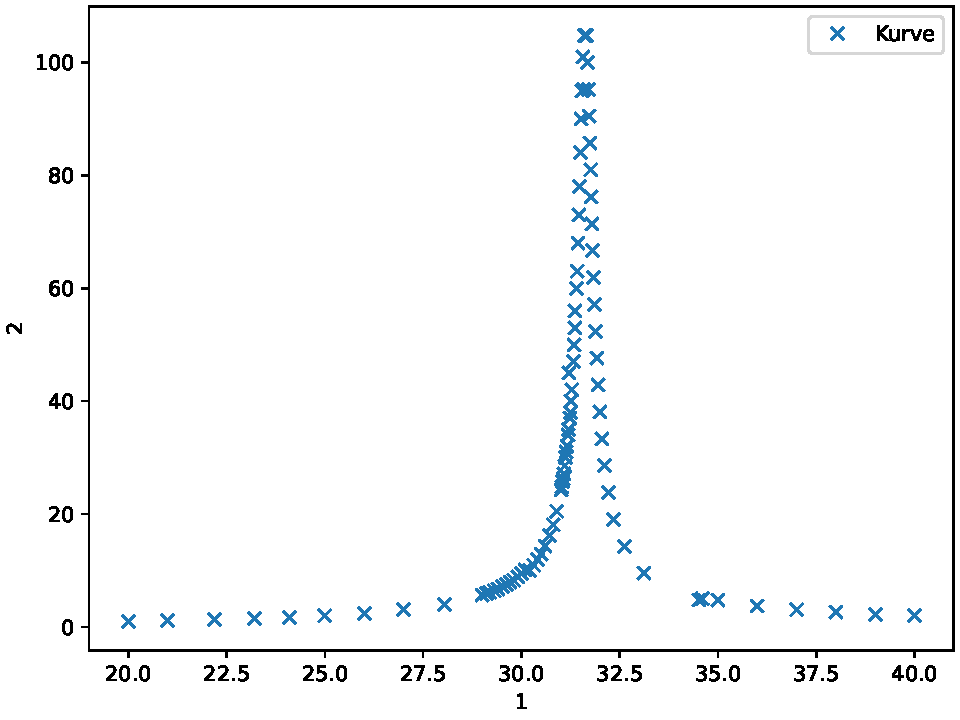
\includegraphics{plot.pdf}
%   \caption{Plot.}
%   \label{fig:plot}
% \end{figure}

%Siehe \autoref{fig:plot}!